\section{Refinement: Flexible fitting}
\label{refinementFlexibleFitting}
Although the rigid fitting approximates map and atomic $model$, a detailed visual inspection of map and model reveals that part of residues are not perfectly fitted. In order to get a better fit, not only of the carbon skeleton but also of residue side chains, a flexible fitting or refinement has to be accomplished. Refinement can thus be defined as the optimization process of fitting $model$ parameters to experimental data. Different strategies can be followed, that can be categorized as refinement in the real space and refinement in Fourier space. Implemented in \scipion are two protocols for real space refinement, \scommand{ccp4 - coot refinement} (Appendix \ref{app:ccp4CootRefinement}, \citep{emsley2010}) and \scommand{phenix - real space refine} (Appendix \ref{app:realSpaceRefineProtocol}, (\citep{afonine2018}), and one protocol to refine in reciprocal space, \scommand{ccp4 - refmac} (Appendix \ref{app:ccp4Refmac}, \citep{vagin2004}).

 \subsection*{CCP4 \coot Refinement}
 
 Initially devoted to atomic models obtained by X-ray crystallography methods, \coot (from Crystallopgraphic Object-Oriented Toolkit) is a 3D computer graphics tool that allows simultaneous display of map and fitted $model$ to accomplish mostly interactive modeling operations. Although this tutorial does not try to show every functionality of \coot, but indicate how to open, close and save partial and final \coot refined structures in \scipion, some of \coot basic relevant commands will be shown. Initially, we are going to refine our \iii{moldel} with \coot. First of all, open \scommand{ccp4 - coot refinement} (\ffigure{fig:coot_refinement_protocol} (1)), load the extracted unit cell volume (2), with electron density normalized to 1, and the fitted structure $model$ (3). Load also the second fit (4) if you are not still sure about the correct fitted structure. Reading the protocol Help is recommended. After executing the protocol (5), \coot graphics window will appear to start working. 
 
 \begin{figure}[H]
  \centering 
  \captionsetup{width=.7\linewidth} 
  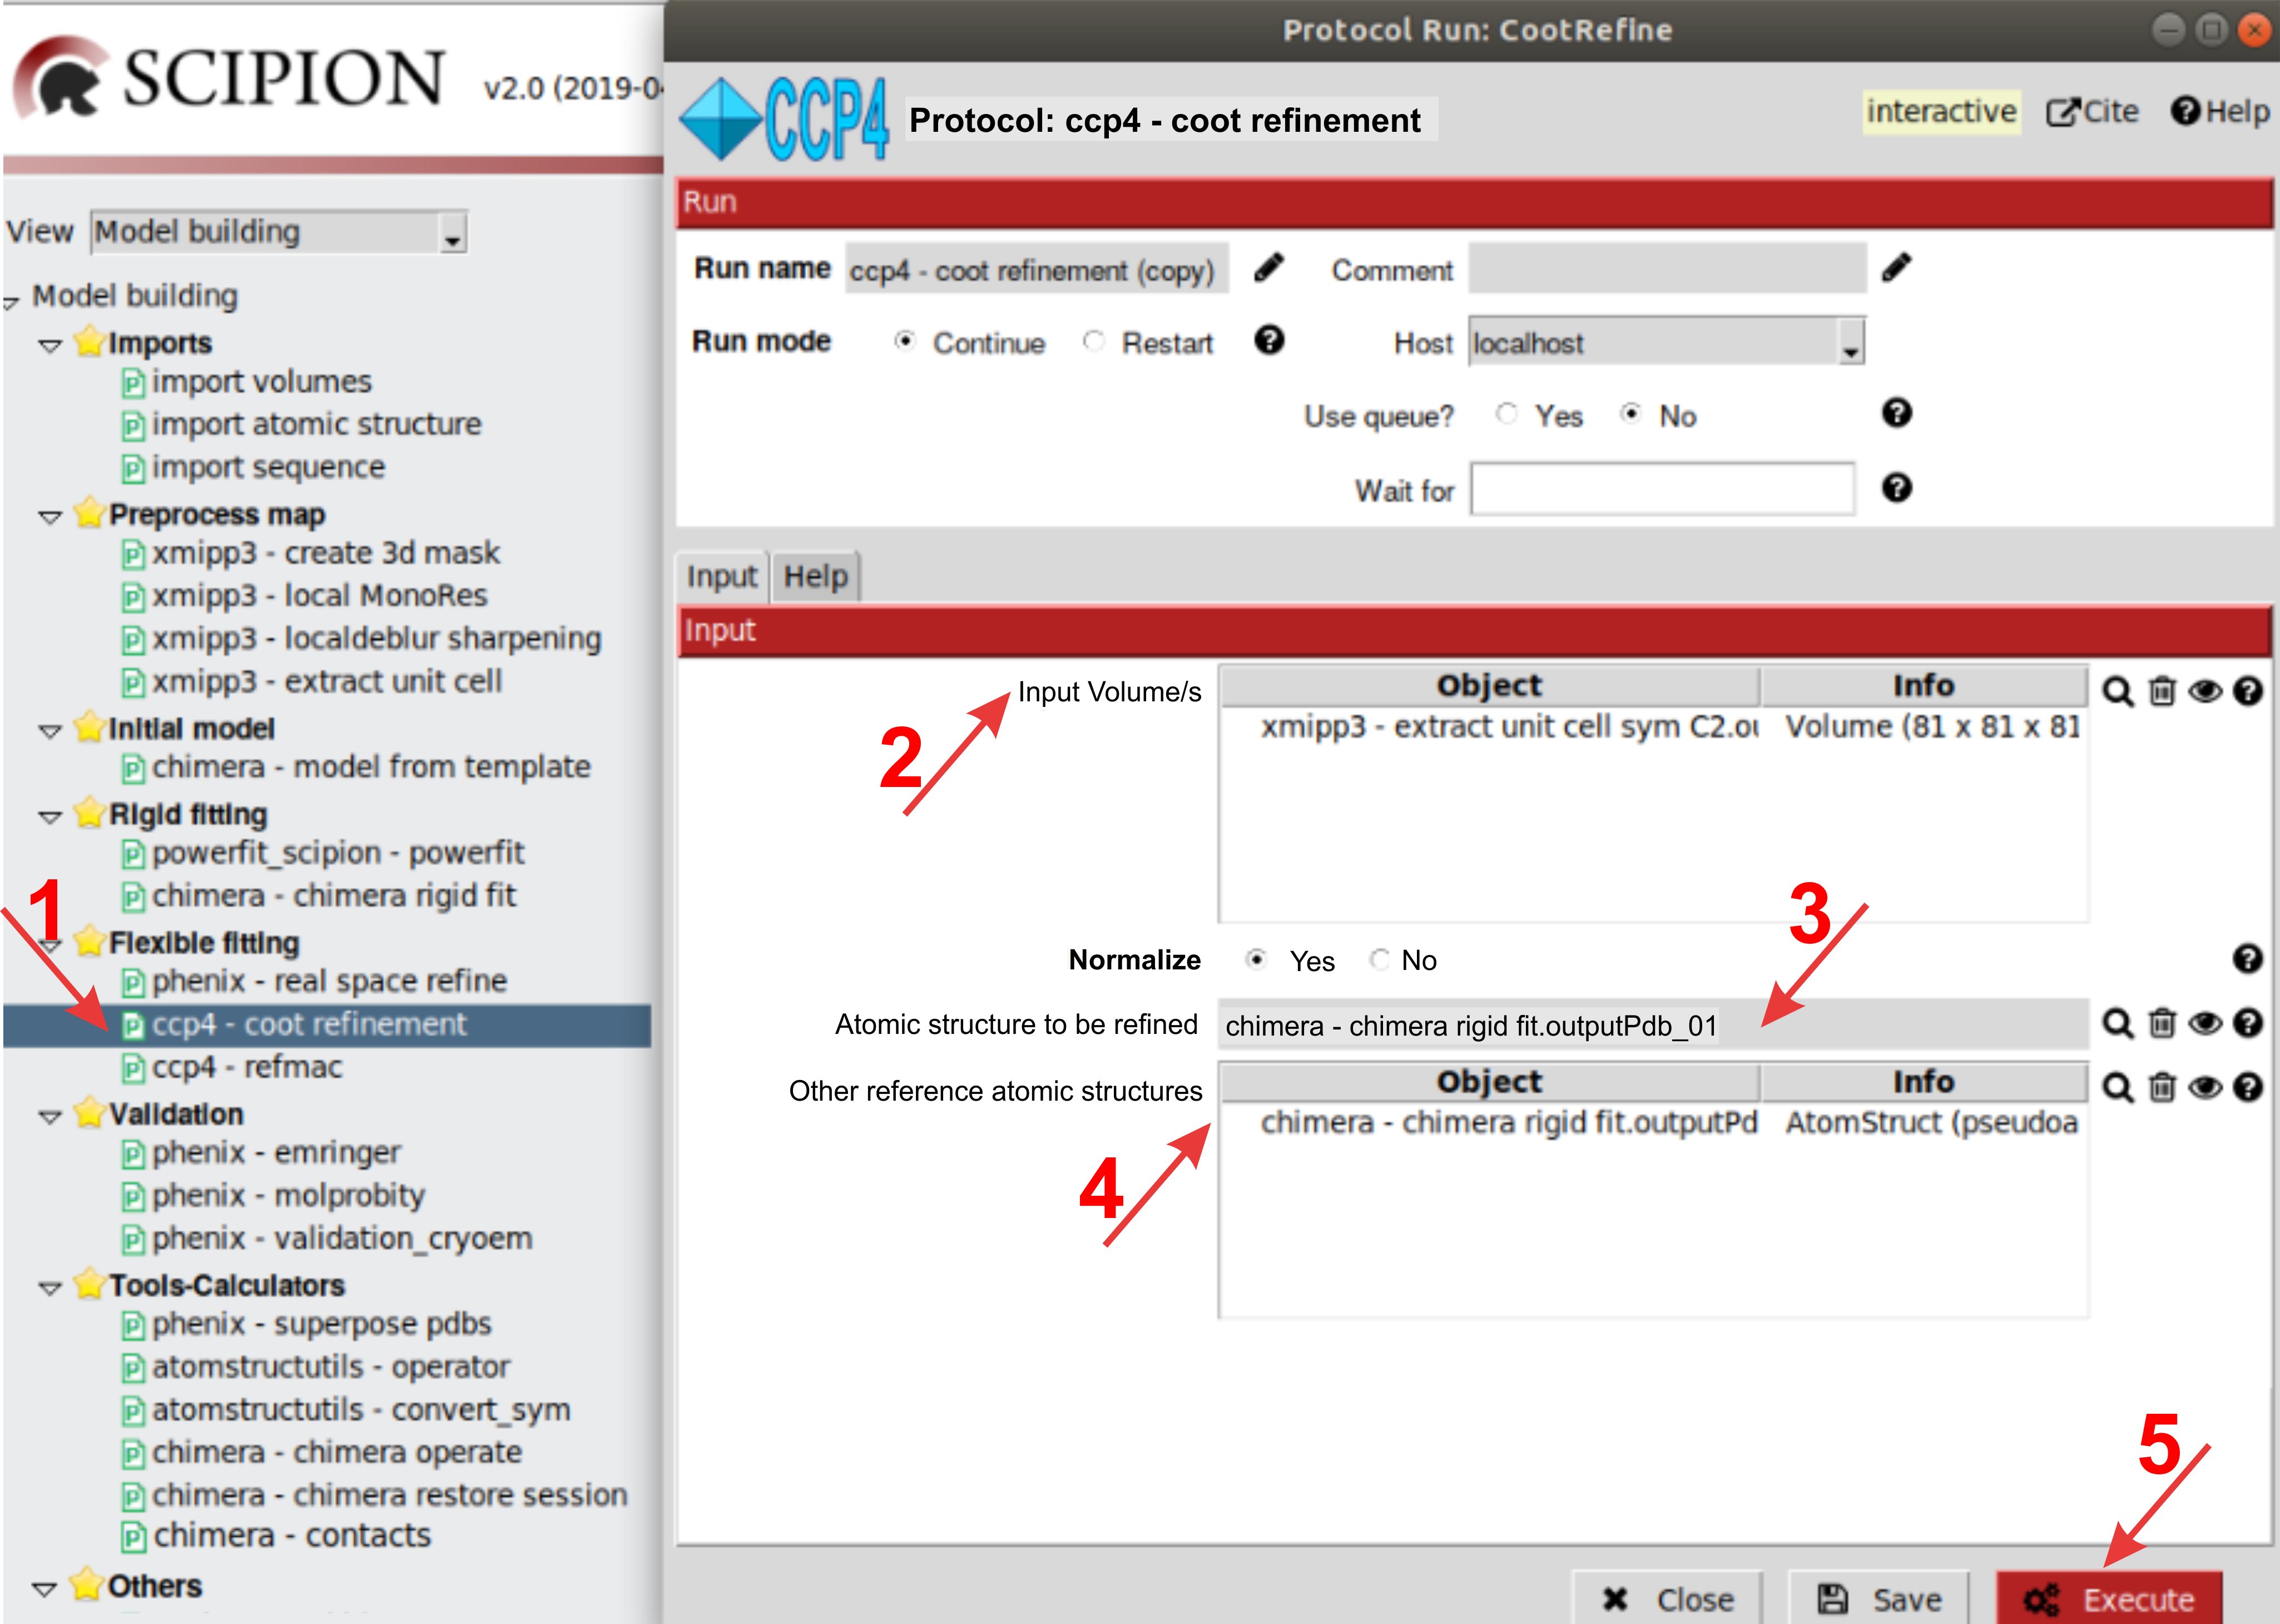
\includegraphics[width=0.85\textwidth]{Images/Fig24}
  \caption{Filling in \coot refinement protocol.}
  \label{fig:coot_refinement_protocol}
  \end{figure}
  

  To check the objects downloaded in \coot, go to the second bar of the main menu and select \ttt{Display Manager}. Map \ttt{(output\_volume.mrc)} (number \ttt{\#2}) and models \ttt{chimeraOut0001.pdb} and \ttt{chimeraOut0002.pdb} (numbers \ttt{\#1} and \ttt{\#0}, respectively) are displayed. To start, we are going to identify the faired fitted $model$ to the density map in order to delete in the \ttt{Display Manager} menu the other $model$, which is misfitted. Visual inspection would clarify this point, although direct observation of the \ttt{Density fit analysis} might be a shorter way. With this aim, go to the main menu of \coot graphical window and select \ttt{Validate -> Density fit analysis}. This density analysis is compared for the two possible fitted \iii{models} in \ffigure{fig:coot_density_fit_analysis}. As you can see, model \ttt{chimeraOut0001.pdb} shows that residues 19, 20 and 22, framed in \ffigure{fig:multiple_alignment_HBB}, do not fit to the density map, as expected from the misfit of the $\alpha$ subunit in the density of the $\beta$ subunit.
 
 \begin{figure}[H]
  \centering 
  \captionsetup{width=.7\linewidth} 
  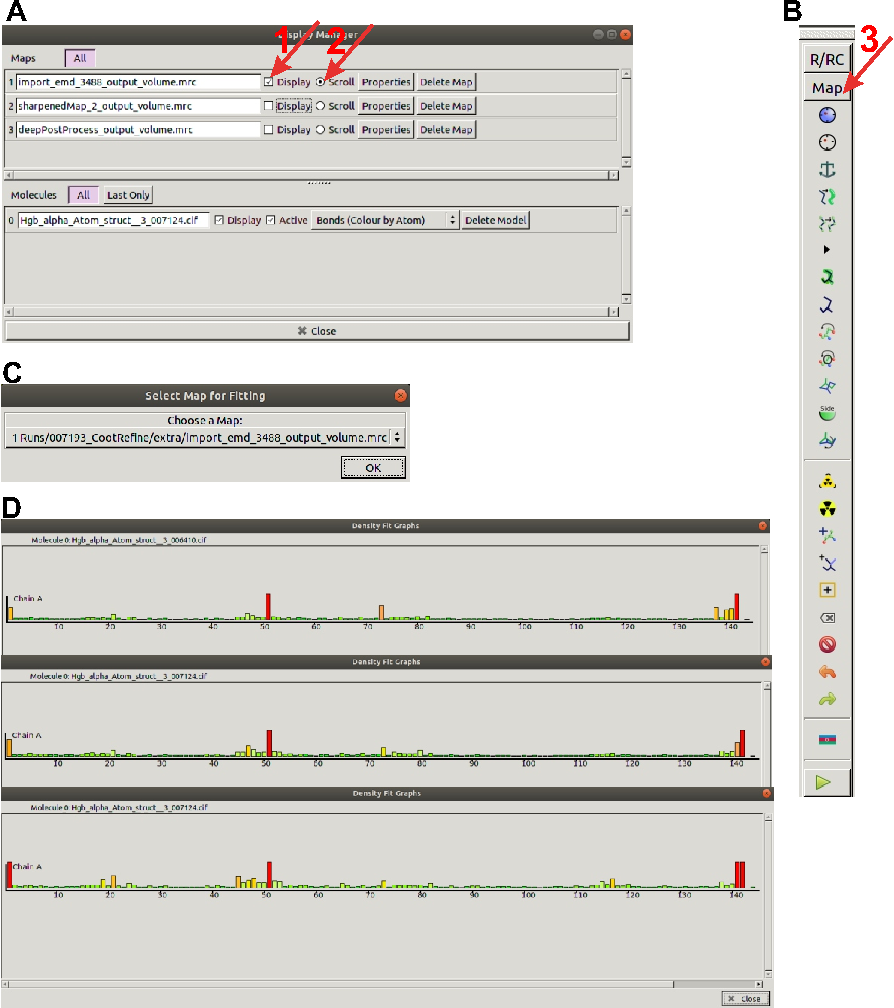
\includegraphics[width=0.85\textwidth]{Images/Fig25}
  \caption{\coot comparison of \iii{model} fit in the map density.}
  \label{fig:coot_density_fit_analysis}
  \end{figure}
  
  Go again to \ttt{Display Manager} and delete the \iii{model} \ttt{chimeraOut0001.pdb} pressing \ttt{Delete Model}. From now ahead, the \iii{model} \ttt{chimeraOut0002.pdb} will be refined in the next steps of the modeling workflow.\\
  
  Before starting the refinement, IDs of chains should be fixed. Current IDs of chains are \ttt{Chain A} and \ttt{Chain} (see \ffigure{fig:coot_density_fit_analysis}) and will be changed to \ttt{Chain HEME} and \ttt{Chain A}, respectively. This can be carried out going to main \coot menu and selecting \ttt{Edit -> Change Chain IDs}. Verify the identity of your \iii{model} molecule (\ffigure{fig:coot_change_name_ID} (1), select the initial Chain ID (2, 4), and write the new Chain ID (3, 5). Finally, press \ttt{Apply New Chain ID}.
 
 \begin{figure}[H]
  \centering 
  \captionsetup{width=.7\linewidth} 
  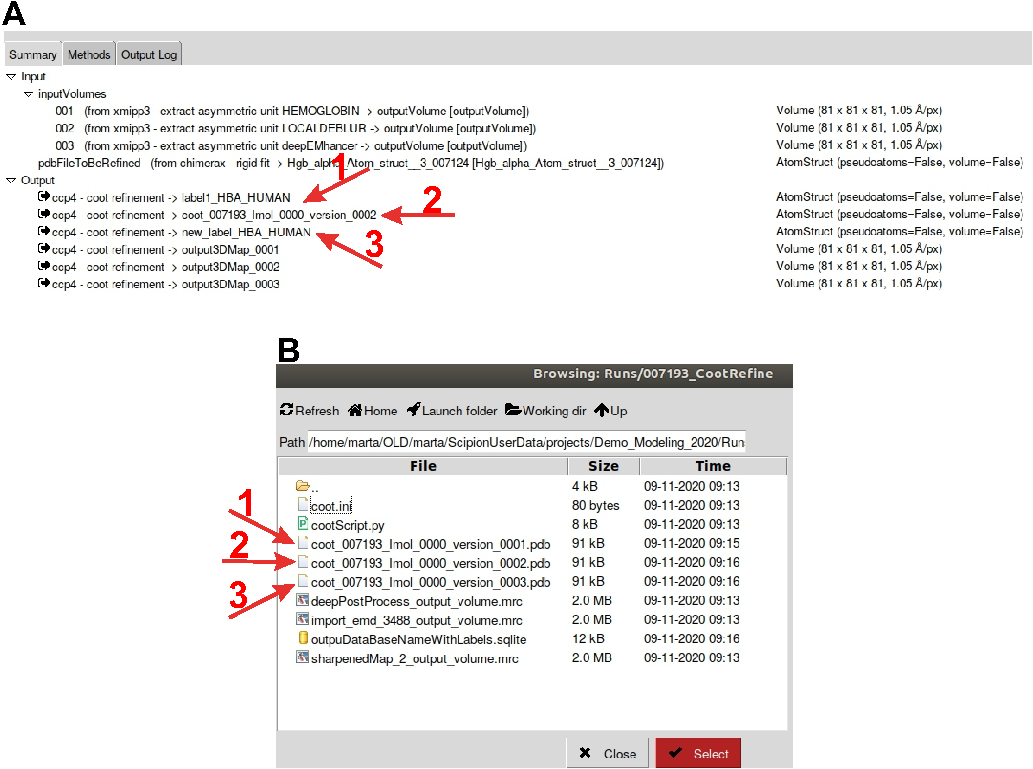
\includegraphics[width=0.85\textwidth]{Images/Fig26}
  \caption{\coot change chain ID of \iii{model} \ttt{chimeraOut0002.pdb}.}
  \label{fig:coot_change_name_ID}
  \end{figure}
  
  According to \ffigure{fig:coot_density_fit_analysis}, \ttt{MET} residue of the new chain \ttt{A} does not fit to the map density. Maybe this residue has been processed post-translationally, as we have anticipated in \textbf{Starting Input data} section. To solve this question, go to \coot main menu and select \ttt{Draw -> Go To Atom... -> Chain A -> A 1 MET} (\ffigure{fig:coot_go_to_atom} (A)). \ttt{MET} residue will be located in the center of \coot graphics widow. Check if this residue is surrounded by any electron density. As \ffigure{fig:coot_go_to_atom} (B)(1) shows, no density associates to the first chain residue. \ttt{MET} will thus be deleted. Then go to the lower right side menu and select the symbol to delete items (B)(2). Select \ttt{Residue/Monomer} in the opened \ttt{Delete item} window, and click the \ttt{MET} residue that you want to delete. Go again to \ttt{Validate -> Density fit analysis} and check that the red bar shown in \ttt{MET} residue (\ffigure{fig:coot_density_fit_analysis}) has disappeared.
  
  \begin{figure}[H]
  \centering 
  \captionsetup{width=.7\linewidth} 
  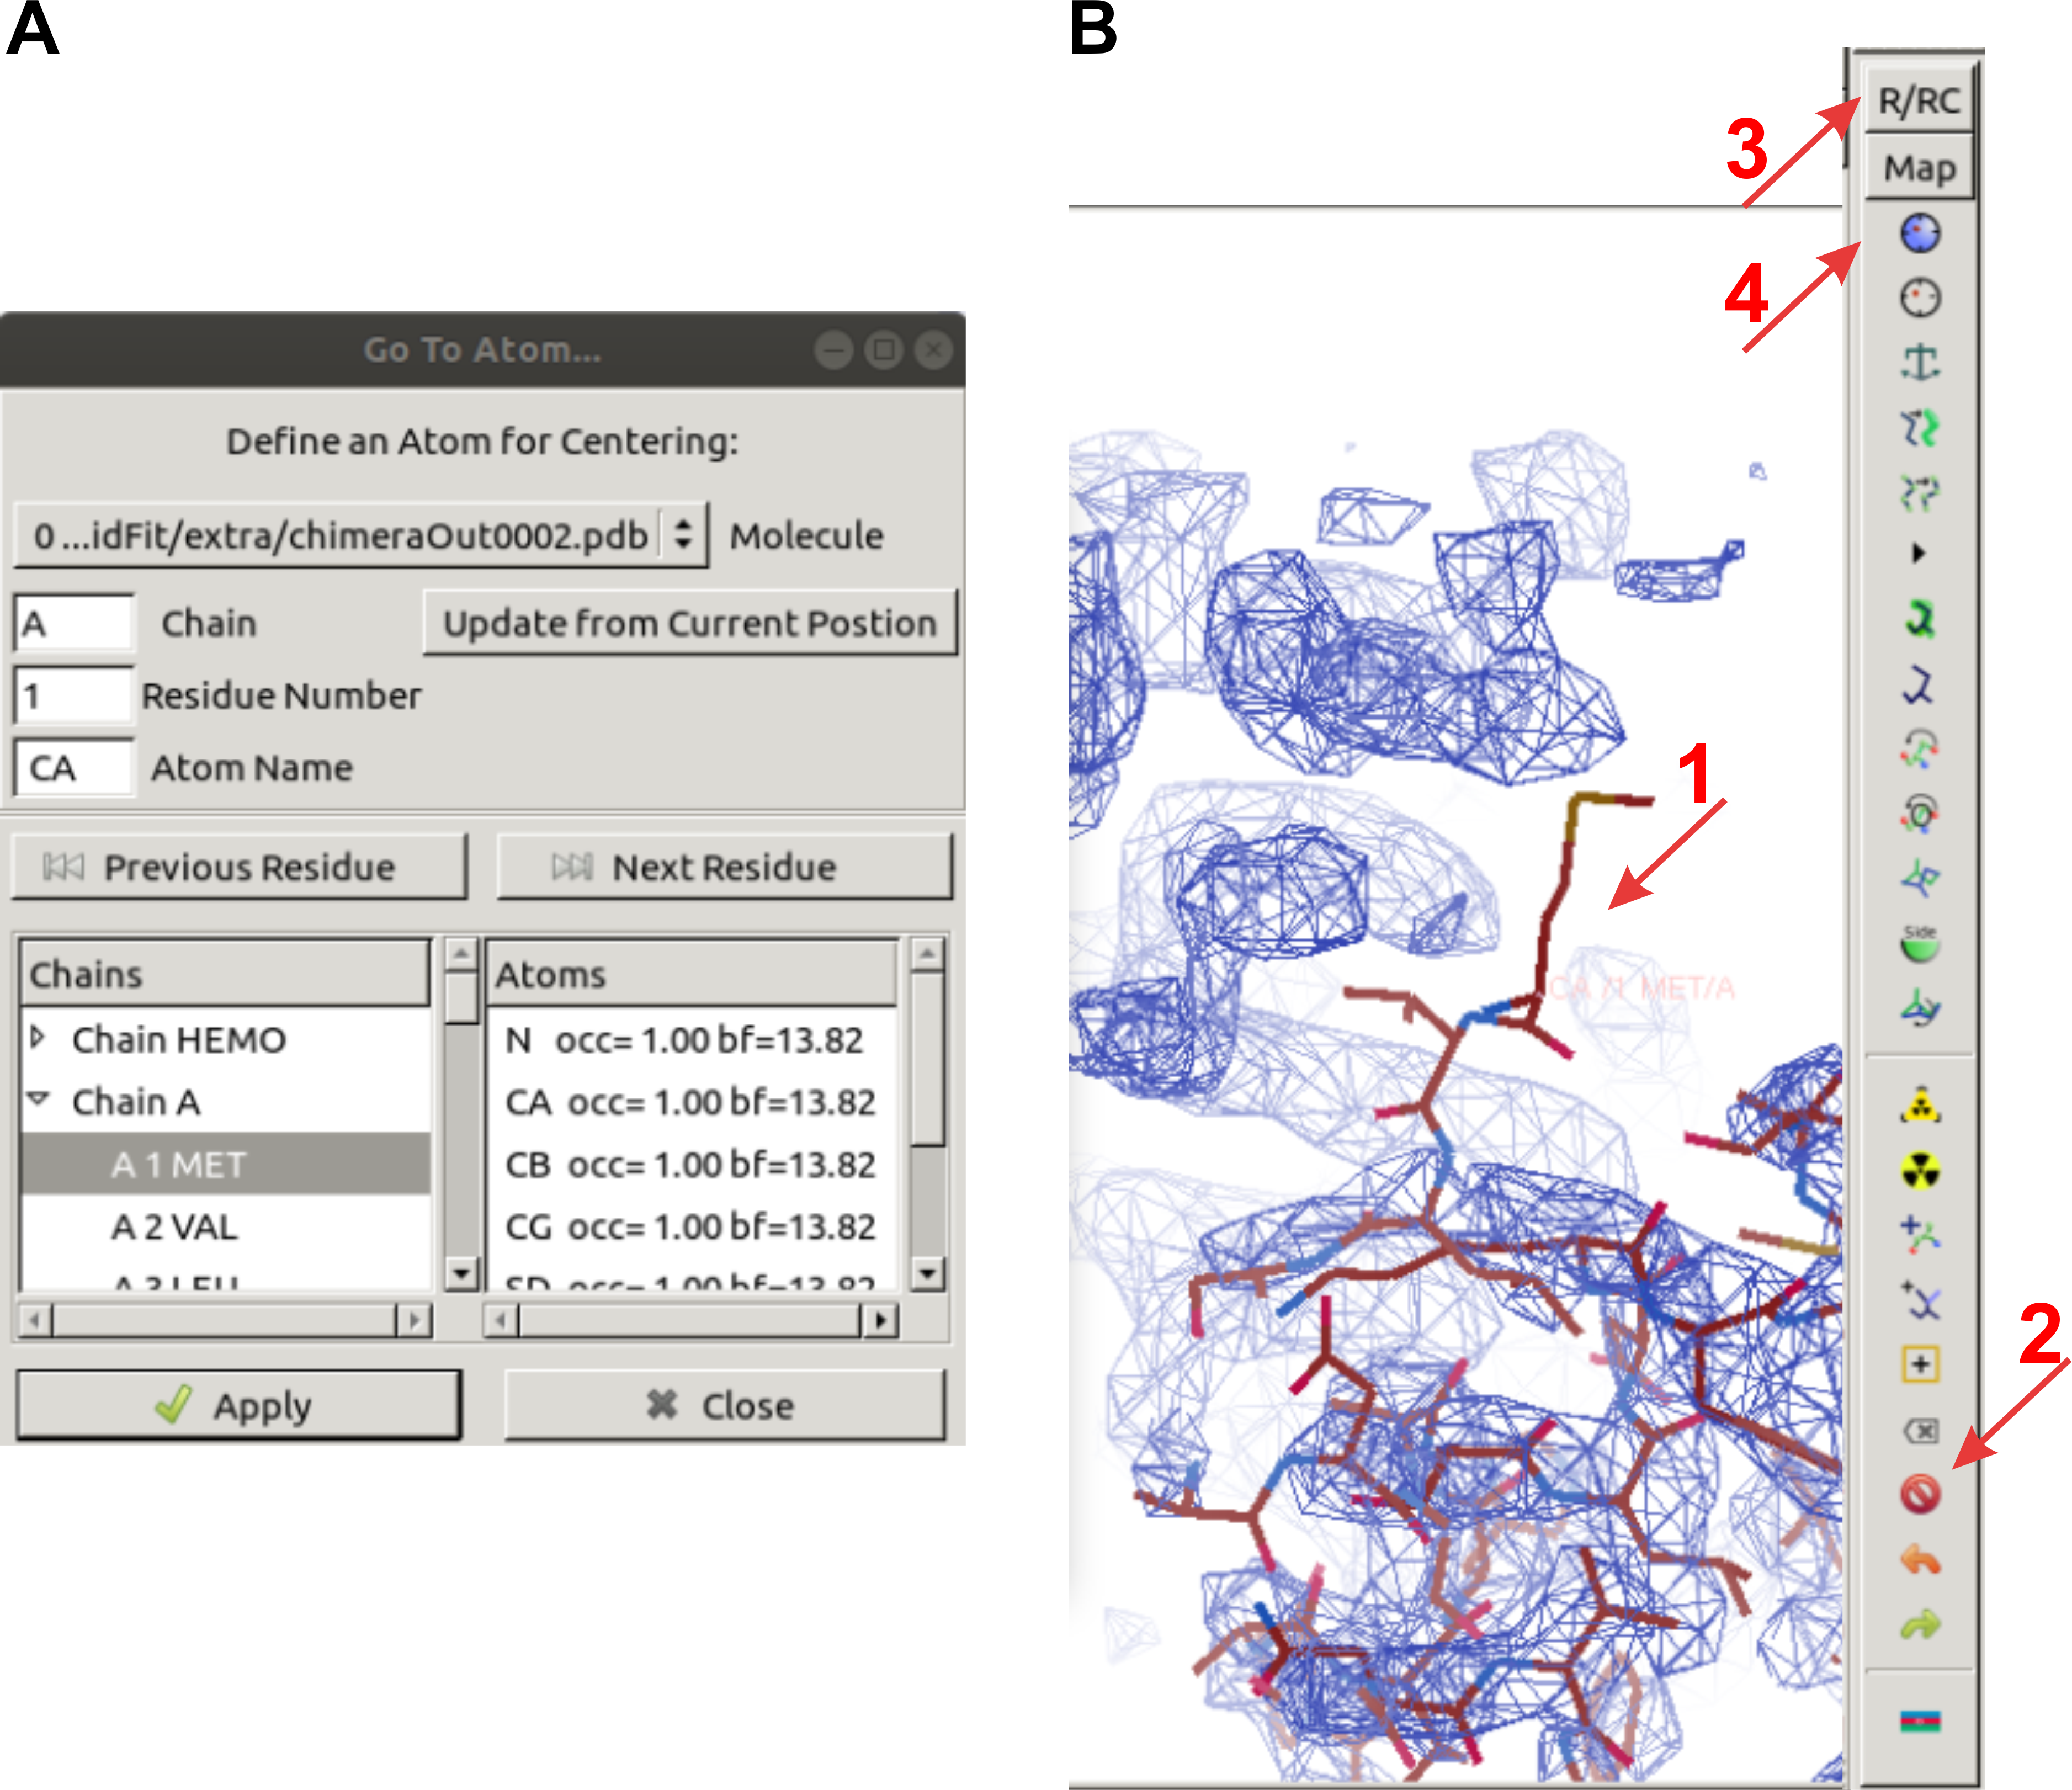
\includegraphics[width=0.80\textwidth]{Images/Fig27}
  \caption{Removing post-translationally processed Methionine residue in \coot. Note that the icons shown in the image right side may be partially hidden if the screen is small}
  \label{fig:coot_go_to_atom}
  \end{figure}
  
  Before a more detailed visual inspection of the \iii{model} fitting, an initial quick refinement may be accomplished. With this purpose, first of all, go to the upper right side menu (\ffigure{fig:coot_go_to_atom} (B)(3)) and select all four restrictions for \ttt{Regularization and Refinement} in the respective window of parameters. Secondly, open the \ttt{coot.ini} text file, 
  open \scipion browser and navigate to the ttt{extra} directory, Modify the file so it match the information shown indicated below. (See \ffigure{fig:cootini}\\
  \ttt{[myvars]}\\
  \ttt{imol: 0}\\
  \ttt{aa\_main\_chain: A}\\
  \ttt{aa\_auxiliary\_chain: AA}\\
  \ttt{aaNumber: 4}\\
  \ttt{step: 10}\\
  
  \begin{figure}[H]
  \centering 
  \captionsetup{width=.7\linewidth} 
  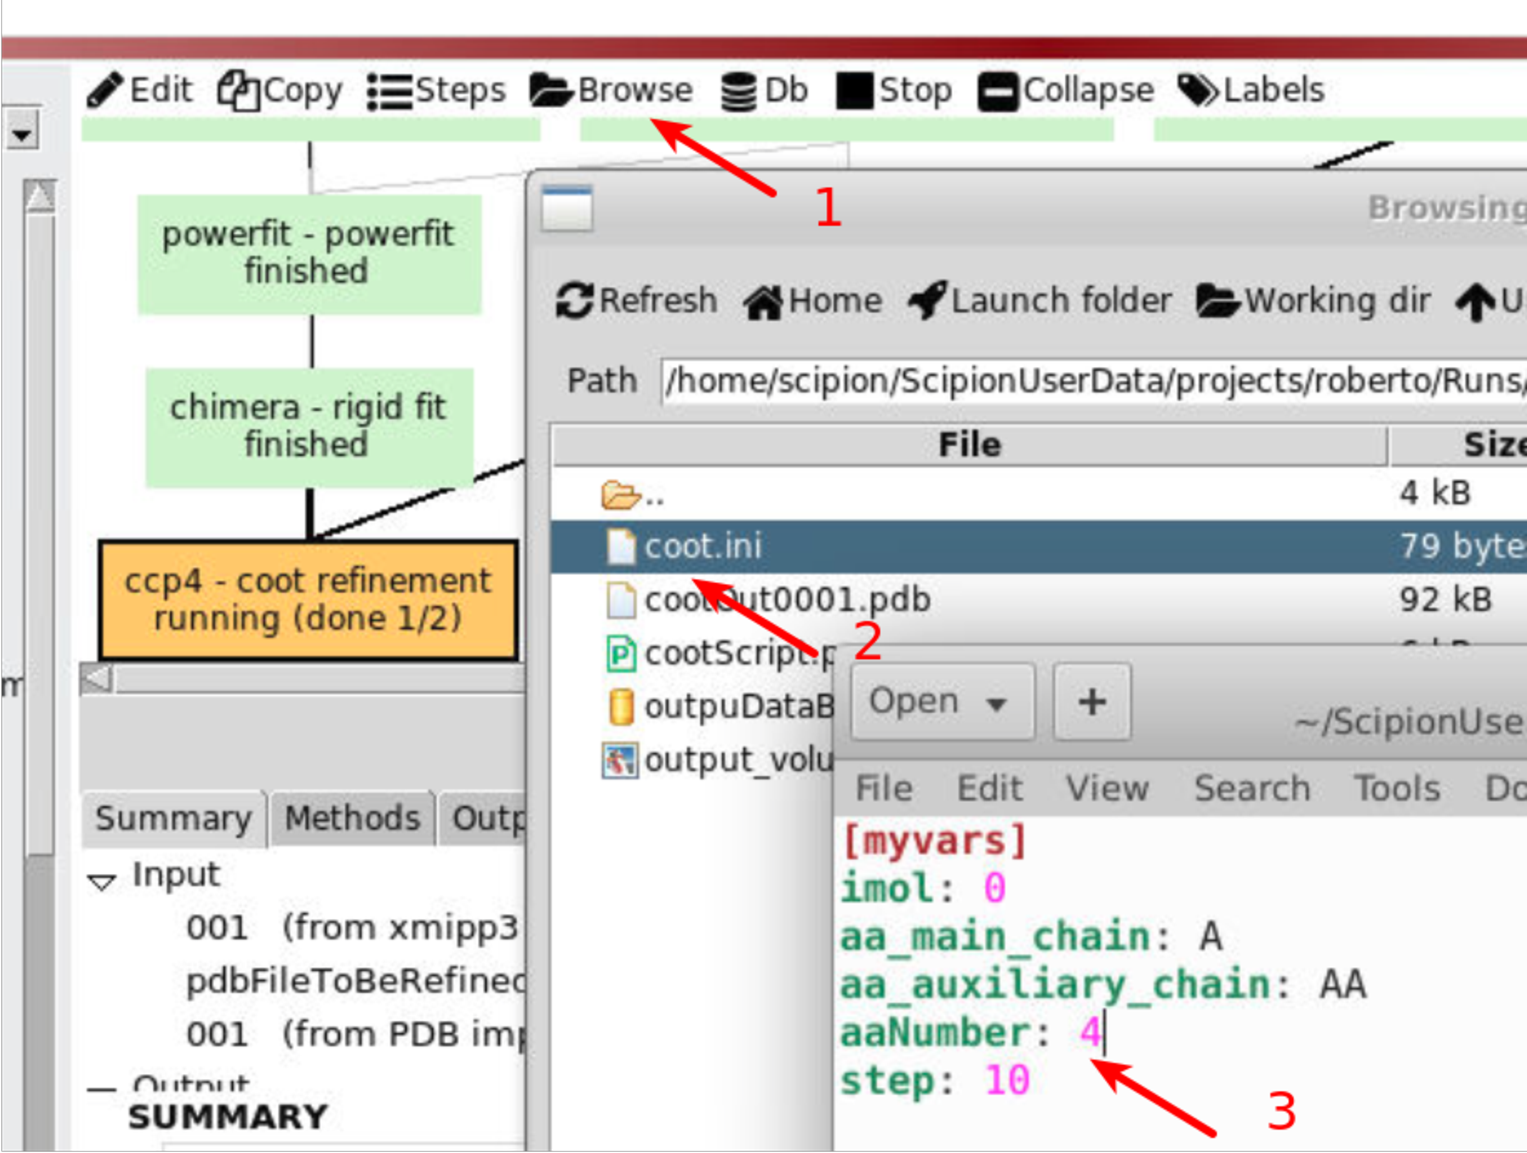
\includegraphics[width=0.80\textwidth]{Images/cootini}
  \caption{Edit coot.ini file.}
  \label{fig:cootini}
  \end{figure}
  
 %[**ROB coot need a careful presentation]
 %[**ROB preguntar a ERney por su metodo de filtracion]
 Finally, go back to \coot window and press ``U'' to initiate global variables and ``z'' to refine the next upstream 10 residues. Go through those residues, one by one, and accept refinement if you agree with it. If you disagree with the refinement of any residue, perform the interactive refinement, visualizing the residue side chain. Repeat the refinement process with ``z'' until the end of the molecule. Check that the orange bar of residue number 50 (\ffigure{fig:coot_density_fit_analysis}) goes missing at the end of this process.\\
 
 After this partially automatic and partially interactive processing, go to \ttt{Draw -> Go To Atom... -> Chain A -> A 2 VAL} (\ttt{VAL} is now the first residue of the \ttt{metHgb} $\alpha$ subunit) and start the detailed interactive refinement of the initial residues of chain A. To accomplish this interactive refinement of a small group of 5 to 10 residues, select the blue circle in the upper right side menu and click the initial and final residues of the small group of residues (\ffigure{fig:coot_go_to_atom} (B)(4)). The group of selected residues gets flexible enough to look manually for another spatial distribution. Following these instructions, try to solve the misfit that you can find in \ttt{TYR} 141 residue at the end of the molecule. Specifically, try to improve the result of the \ttt{Validate -> Density fit analysis}, as you can see from (A) to (B) in \ffigure{fig:coot_density_fit_analysis2}, moving \ttt{TYR} 141 ((A)(1)) to the nearest empty map density ((A)(2)). Accept the refinement parameters after the displacement of \ttt{TYR} ((B)(3)). Finally, check the \ttt{Density Fit Graph}.
 
  \begin{figure}[H]
  \centering 
  \captionsetup{width=.7\linewidth} 
  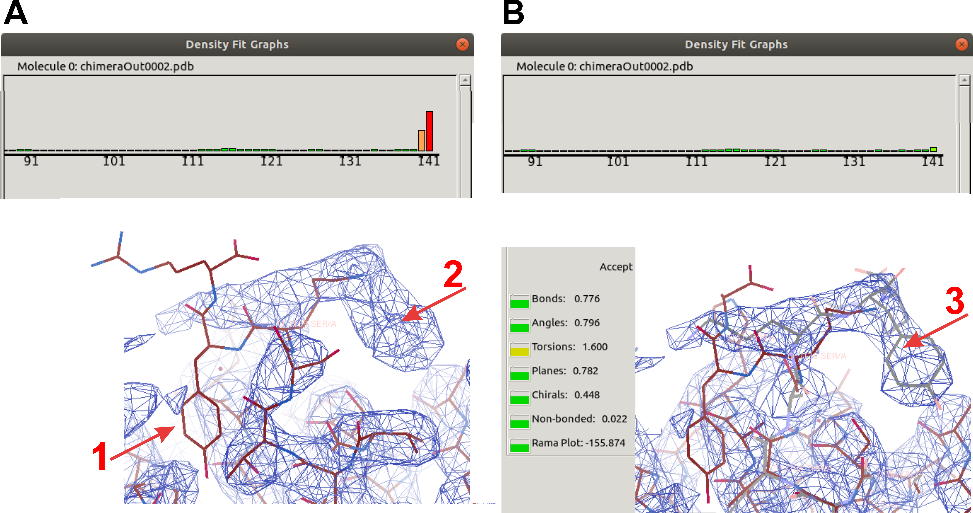
\includegraphics[width=0.85\textwidth]{Images/Fig28}
  \caption{\coot fit in the map density of residue \ttt{TYR} 141.}
  \label{fig:coot_density_fit_analysis2}
  \end{figure}
  
 Rotamer refinement is another refinement tool available in \coot. You can try to improve your current $model$ modifying rotamers reported as incorrect in \ttt{Validate -> Rotamer analysis}. Otherwise, the next refinement program in modeling workflow (\phenix \ttt{real space refine}) will perform rotamer refinement.\\
 
 At the end of this interactive refinement with \coot, the refined atomic structure has to be saved. You can save the atomic structure with its default name by pressing \keys{w}. If you prefer another name, for instance ``HBA\_HUMAN.pdb'', it can be saved in \coot main menu \ttt{Calculate -> Scripting -> Python} and the \ttt{Coot Python Scripting} window will be opened. Assuming that \ttt{0} is your \iii{model} number, write in Command:\\
 \ttt{scipion\_write (0, 'HBA\_HUMAN')}\keys{\return}
 
 In its interactive way, \scommand{ccp4 - coot refinement} protocol can be launched again whenever you want in \scipion, and the last atomic structure saved will be loaded in \coot graphics window. This functionality of \scipion allows to stop the interactive refinement and restart the process in the last refinement step, maintaining each one of the intermediate refined structures saved in order in \scipion tutorial folder \ttt{/Runs/000XXX\_CootRefine/extra}. In this way, go again to intermediate refined structures is also possible. Finally, when you reach the final refined structure save it, and you may press \keys{e} to fully stop protocol \coot.\\
 
 A similar refinement process to that followed in \coot for \ttt{metHgb} $\alpha$ subunit chain \ttt{A}, has to be carried out for chain \ttt{HEME} and for respective chains of \ttt{metHgb} $\beta$ subunit.\\
 
 
 \subsection*{\phenix Real Space Refine}
 
 In order to compare the previous \coot interactive refinement with an automatic refinement, we are going to use the
 \scommand{phenix - real space refine} protocol in parallel. This protocol implements in \scipion the \iii{phenix.real\_space\_refine} program developed to address cryo-EM structure-refinement requirements. Following a workflow similar to the \phenix reciprocal-space refinement program \iii{phenix.refine}, basically devoted to crystallography, \iii{phenix.real\_space\_refine} program, mainly used in cryo-EM, is able to refine in real space atomic models against maps, which are the experimental data.\\
 
 Start working by opening \scommand{phenix - real space refine} protocol (\ffigure{fig:phenix_real_space_refine_protocol} (1)), load as input volume the extracted unit cell saved in \coot (2), write the volume resolution (3), load the atomic structure ($model$ \ttt{chimeraOut0002.pdb}, (4)) and select the output format of the refined atomic structure that will be generated (5). After executing the protocol (6), results can be checked (7). 
 
 \begin{figure}[H]
  \centering 
  \captionsetup{width=.7\linewidth} 
  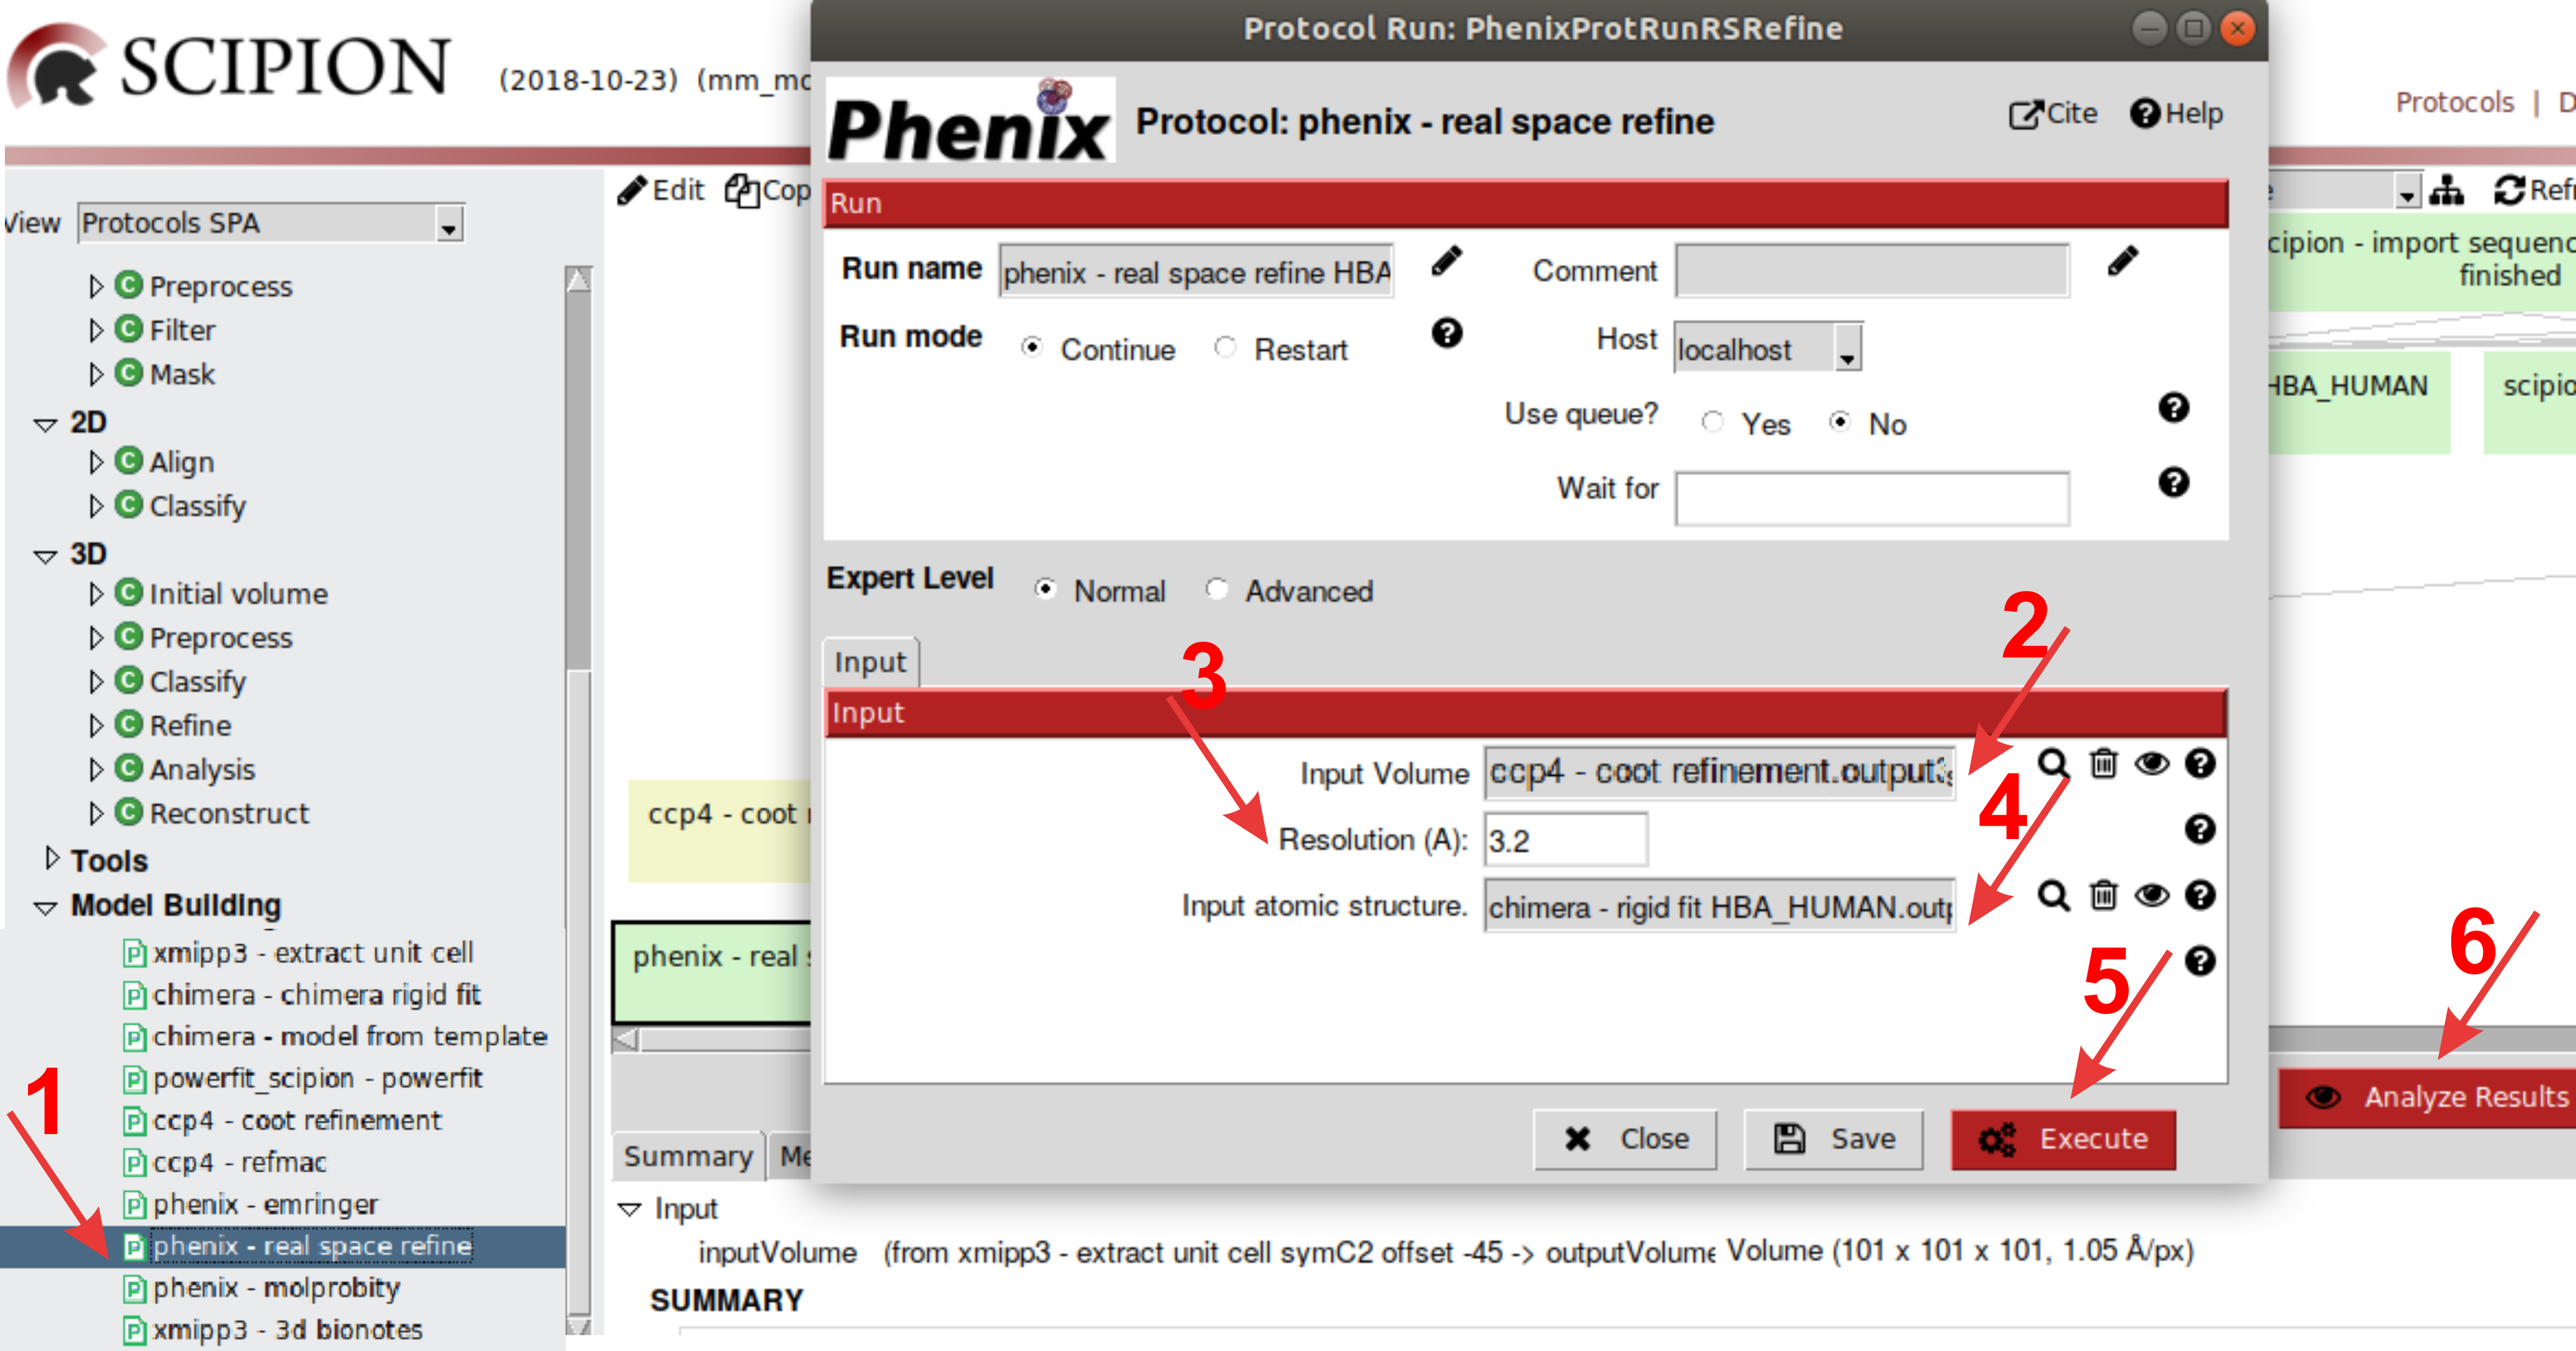
\includegraphics[width=0.85\textwidth]{Images/Fig29}
  \caption{Completing \phenix Real Space Refine protocol.}
  \label{fig:phenix_real_space_refine_protocol}
  \end{figure}
 
 The first tab of results shows the initial $model$ atomic structure as well as the refined one, both fitted to the normalized extract unit cell volume saved in \coot (\ffigure{fig:phenix_real_space_refine_chimera}). 
 
 \begin{figure}[H]
  \centering 
  \captionsetup{width=.7\linewidth} 
  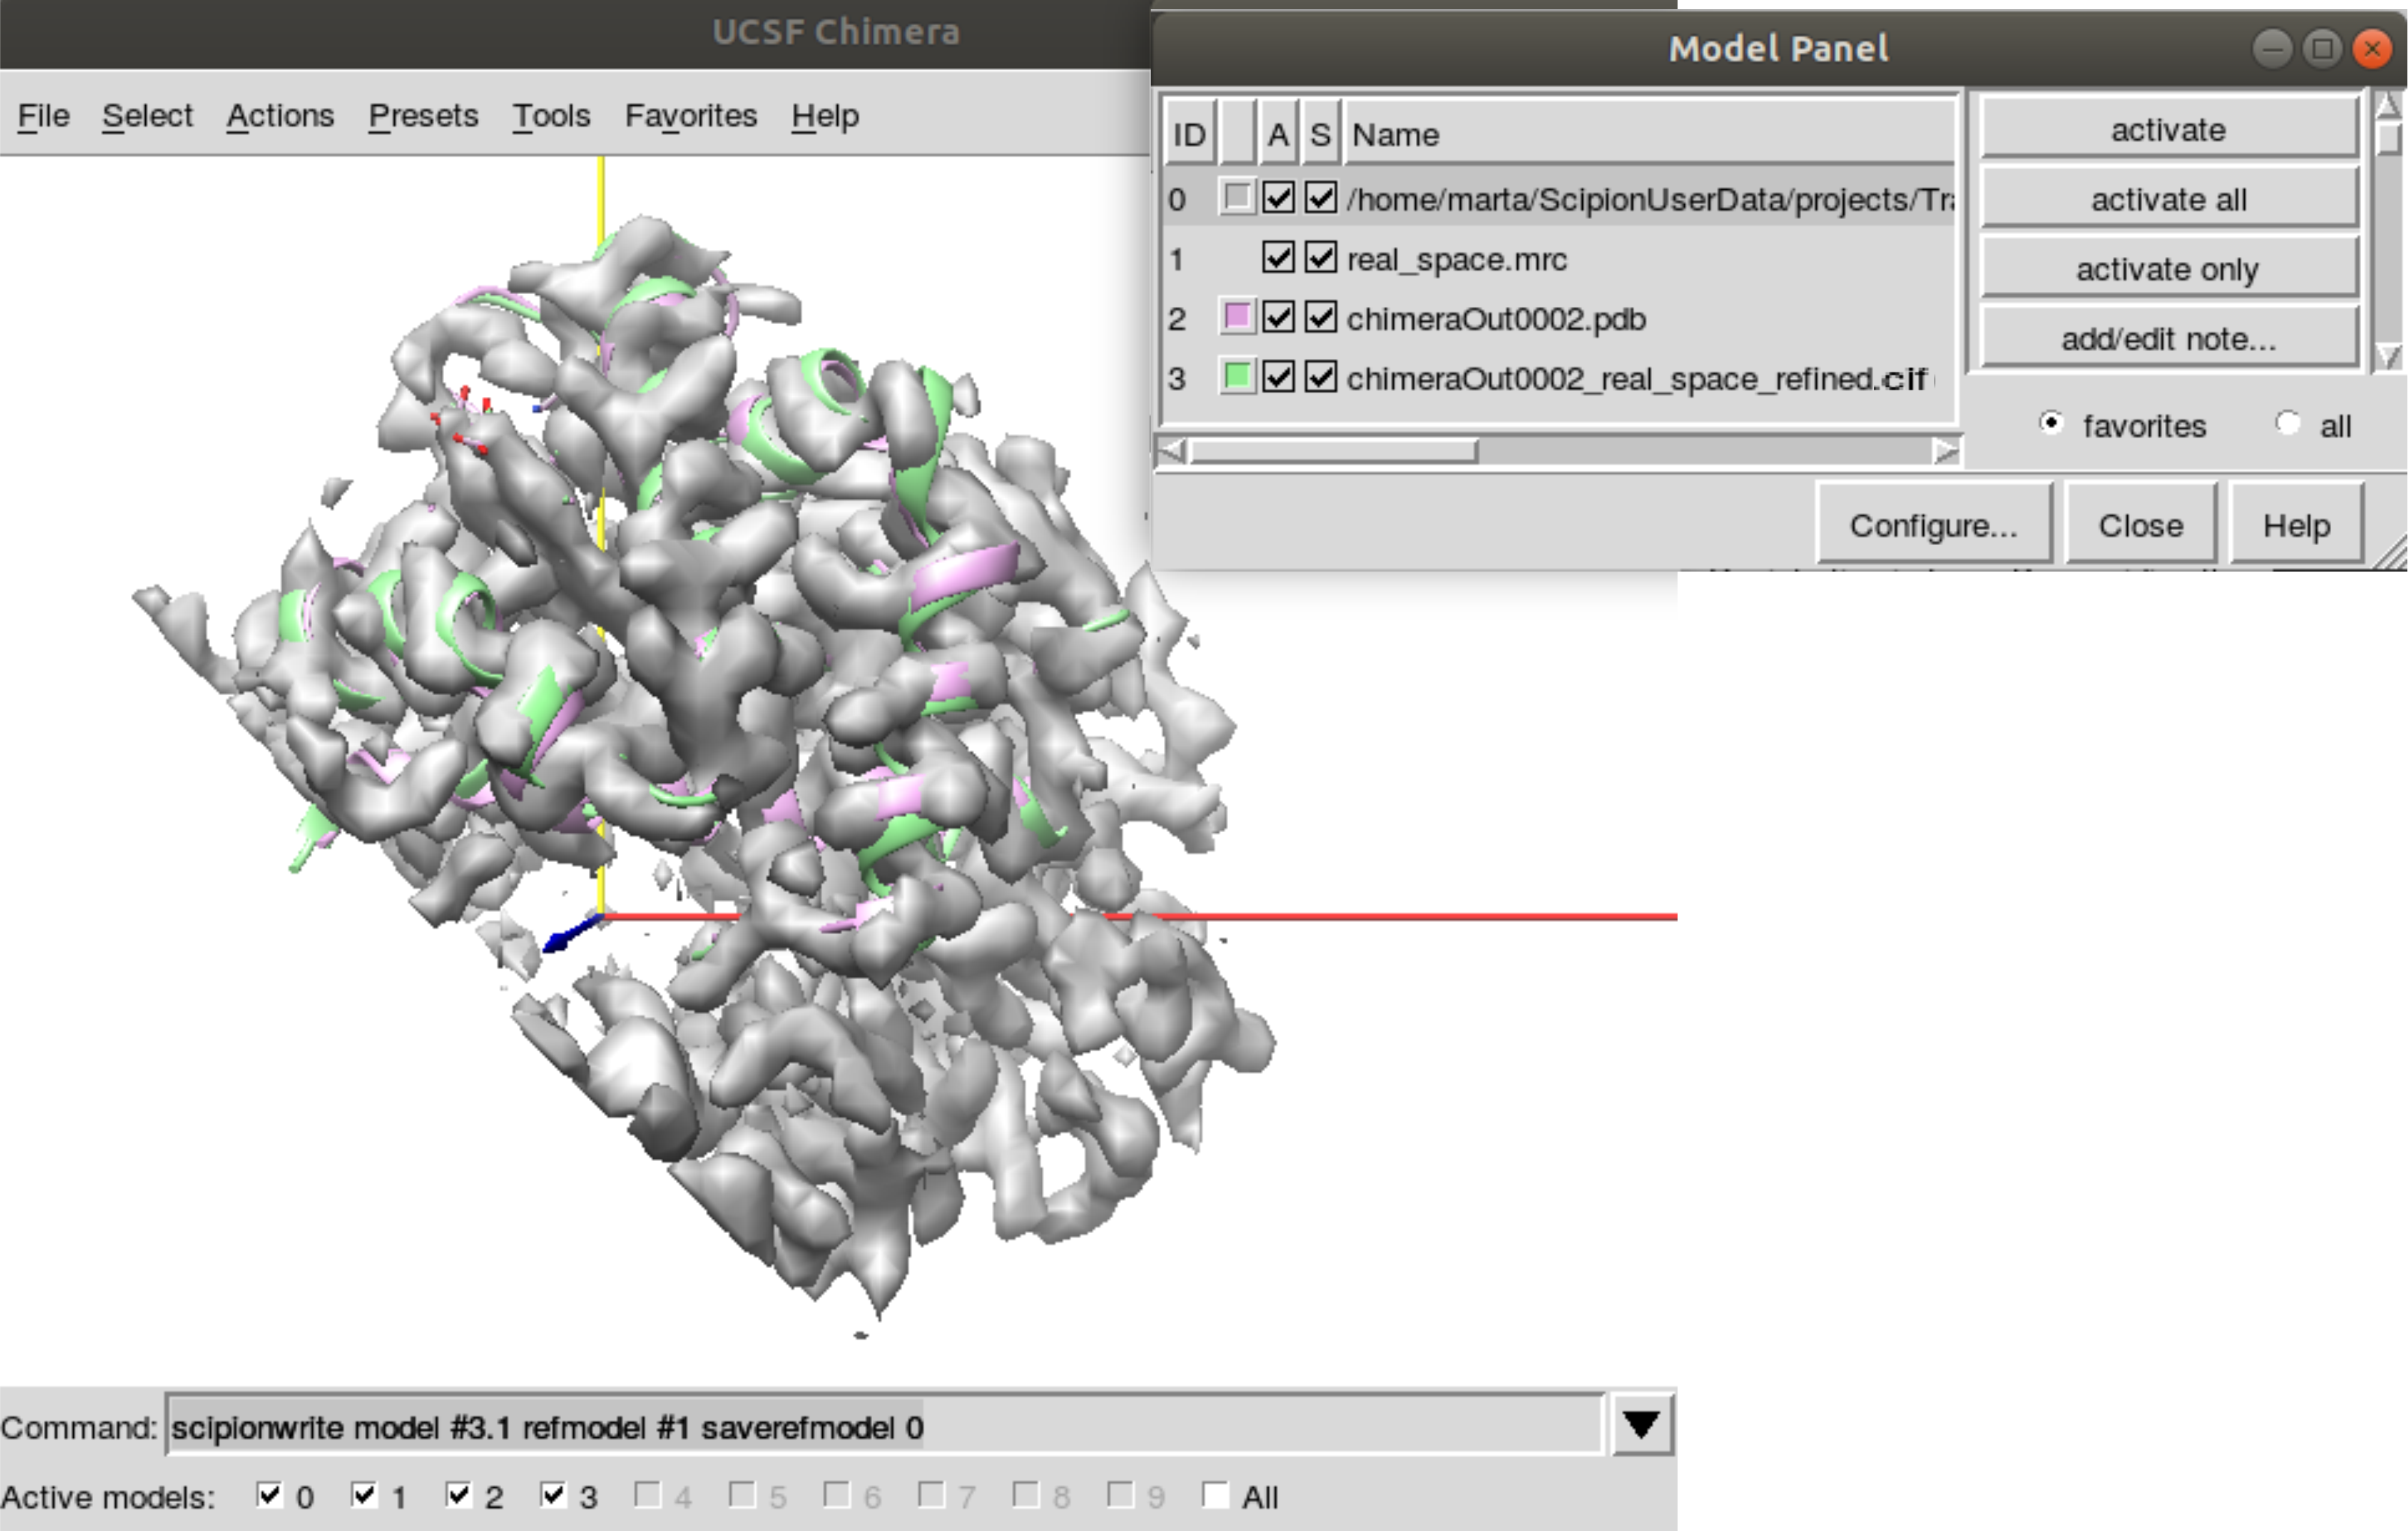
\includegraphics[width=0.85\textwidth]{Images/Fig30}
  \caption{$Chimera$ visualization of refined $model$ of \ttt{metHgb} $\alpha$ subunit by \phenix Real Space Refine protocol.}
  \label{fig:phenix_real_space_refine_chimera}
  \end{figure}
  
  The rest of tabs detail different statistics useful to compare the quality of distinct $models$ such as $MolProbity$ statistics and \ttt{Real-space} correlations. $MolProbity$ results will be discussed in the next section of validation and comparison. Regarding \ttt{Real-space} correlations, different $mdels$ can be compared by using the global number of \ccmask, that indicates the correlation $model$-to-map calculated considering the map region masked around the $model$. You can check also individual correlation values for each residue.  Remark that residues with lower correlation values might be susceptible to improve by additional refinement in \coot. Have a look to those correlation values and answer the following questions: (Answers in appendix \ref{app:solutions}; \textbf{Question \ref{refinementFlexibleFitting}\_1}) \\
  
  \begin{minipage}{\linewidth}
  \begin{framed}
  \begin{itemize}
  \item What is the \ccmask value?
  \item Which one is the residue that shows the lower correlation value? Why?
  \item What is that correlation value?
  \item Which one is the second residue that shows the lower correlation value? Why?
  \item What is that correlation value?
  \item What is the correlation value of \ttt{HEME} group?
  \end{itemize}
  \end{framed}
  \end{minipage}\\
  
  The conclusion of this part of refinement in real space is that \coot and \phenix \ttt{real space refine} might perform complementary tasks. The usage of both protocols may improve the result, especially when partial processing or big arrangements of molecules are involved. Now, to take advance of $model$ improvements performed with \coot, run \phenix \ttt{real space refine} after \coot. When you finish, check again the above values of correlation. Have they changed? (Answer in appendix \ref{app:solutions}; \textbf{Question \ref{refinementFlexibleFitting}\_2})
  
  Before finishing our refinement workflow with \refmac, we can ask ourselves how can we improve correlations in real space by modifying the advance parameters in the protocol form. Will the correlation values change if we set to ``yes'' optimization parameters previously set to ``no'' and increase the number of macro cycles from 5 to 30? Take into account that this process take much more time (around 6 times more) than the previous one. (Answer in appendix \ref{app:solutions}; \textbf{Question \ref{refinementFlexibleFitting}\_3})\\
  
  \subsection*{\ccp4  \refmac}
  
  As in the case of \coot, \refmac (from maximum-likelihood Refinement of Macromolecules) was initially developed to optimize models obtained by X-ray crystallography methods, but unlike \coot, automatically and in reciprocal space. The $models$ refined in the real space with \coot and \phenix \ttt{real space refine}, successively, will be used as input to perform a second refinement step in the Fourier space with \refmac protocol \scommand{ccp4 - refmac}. Firstly, open the \refmac protocol form (\ffigure{fig:refmac_protocol} (1)), load the volume generated by \coot (2), the atomic structure obtained with \phenix \ttt{real space refine} (3), and the volume resolution as maximum resolution (4). Execute the protocol (5) and when it finish, analyze the results (6).
  
  \begin{figure}[H]
  \centering 
  \captionsetup{width=.7\linewidth} 
  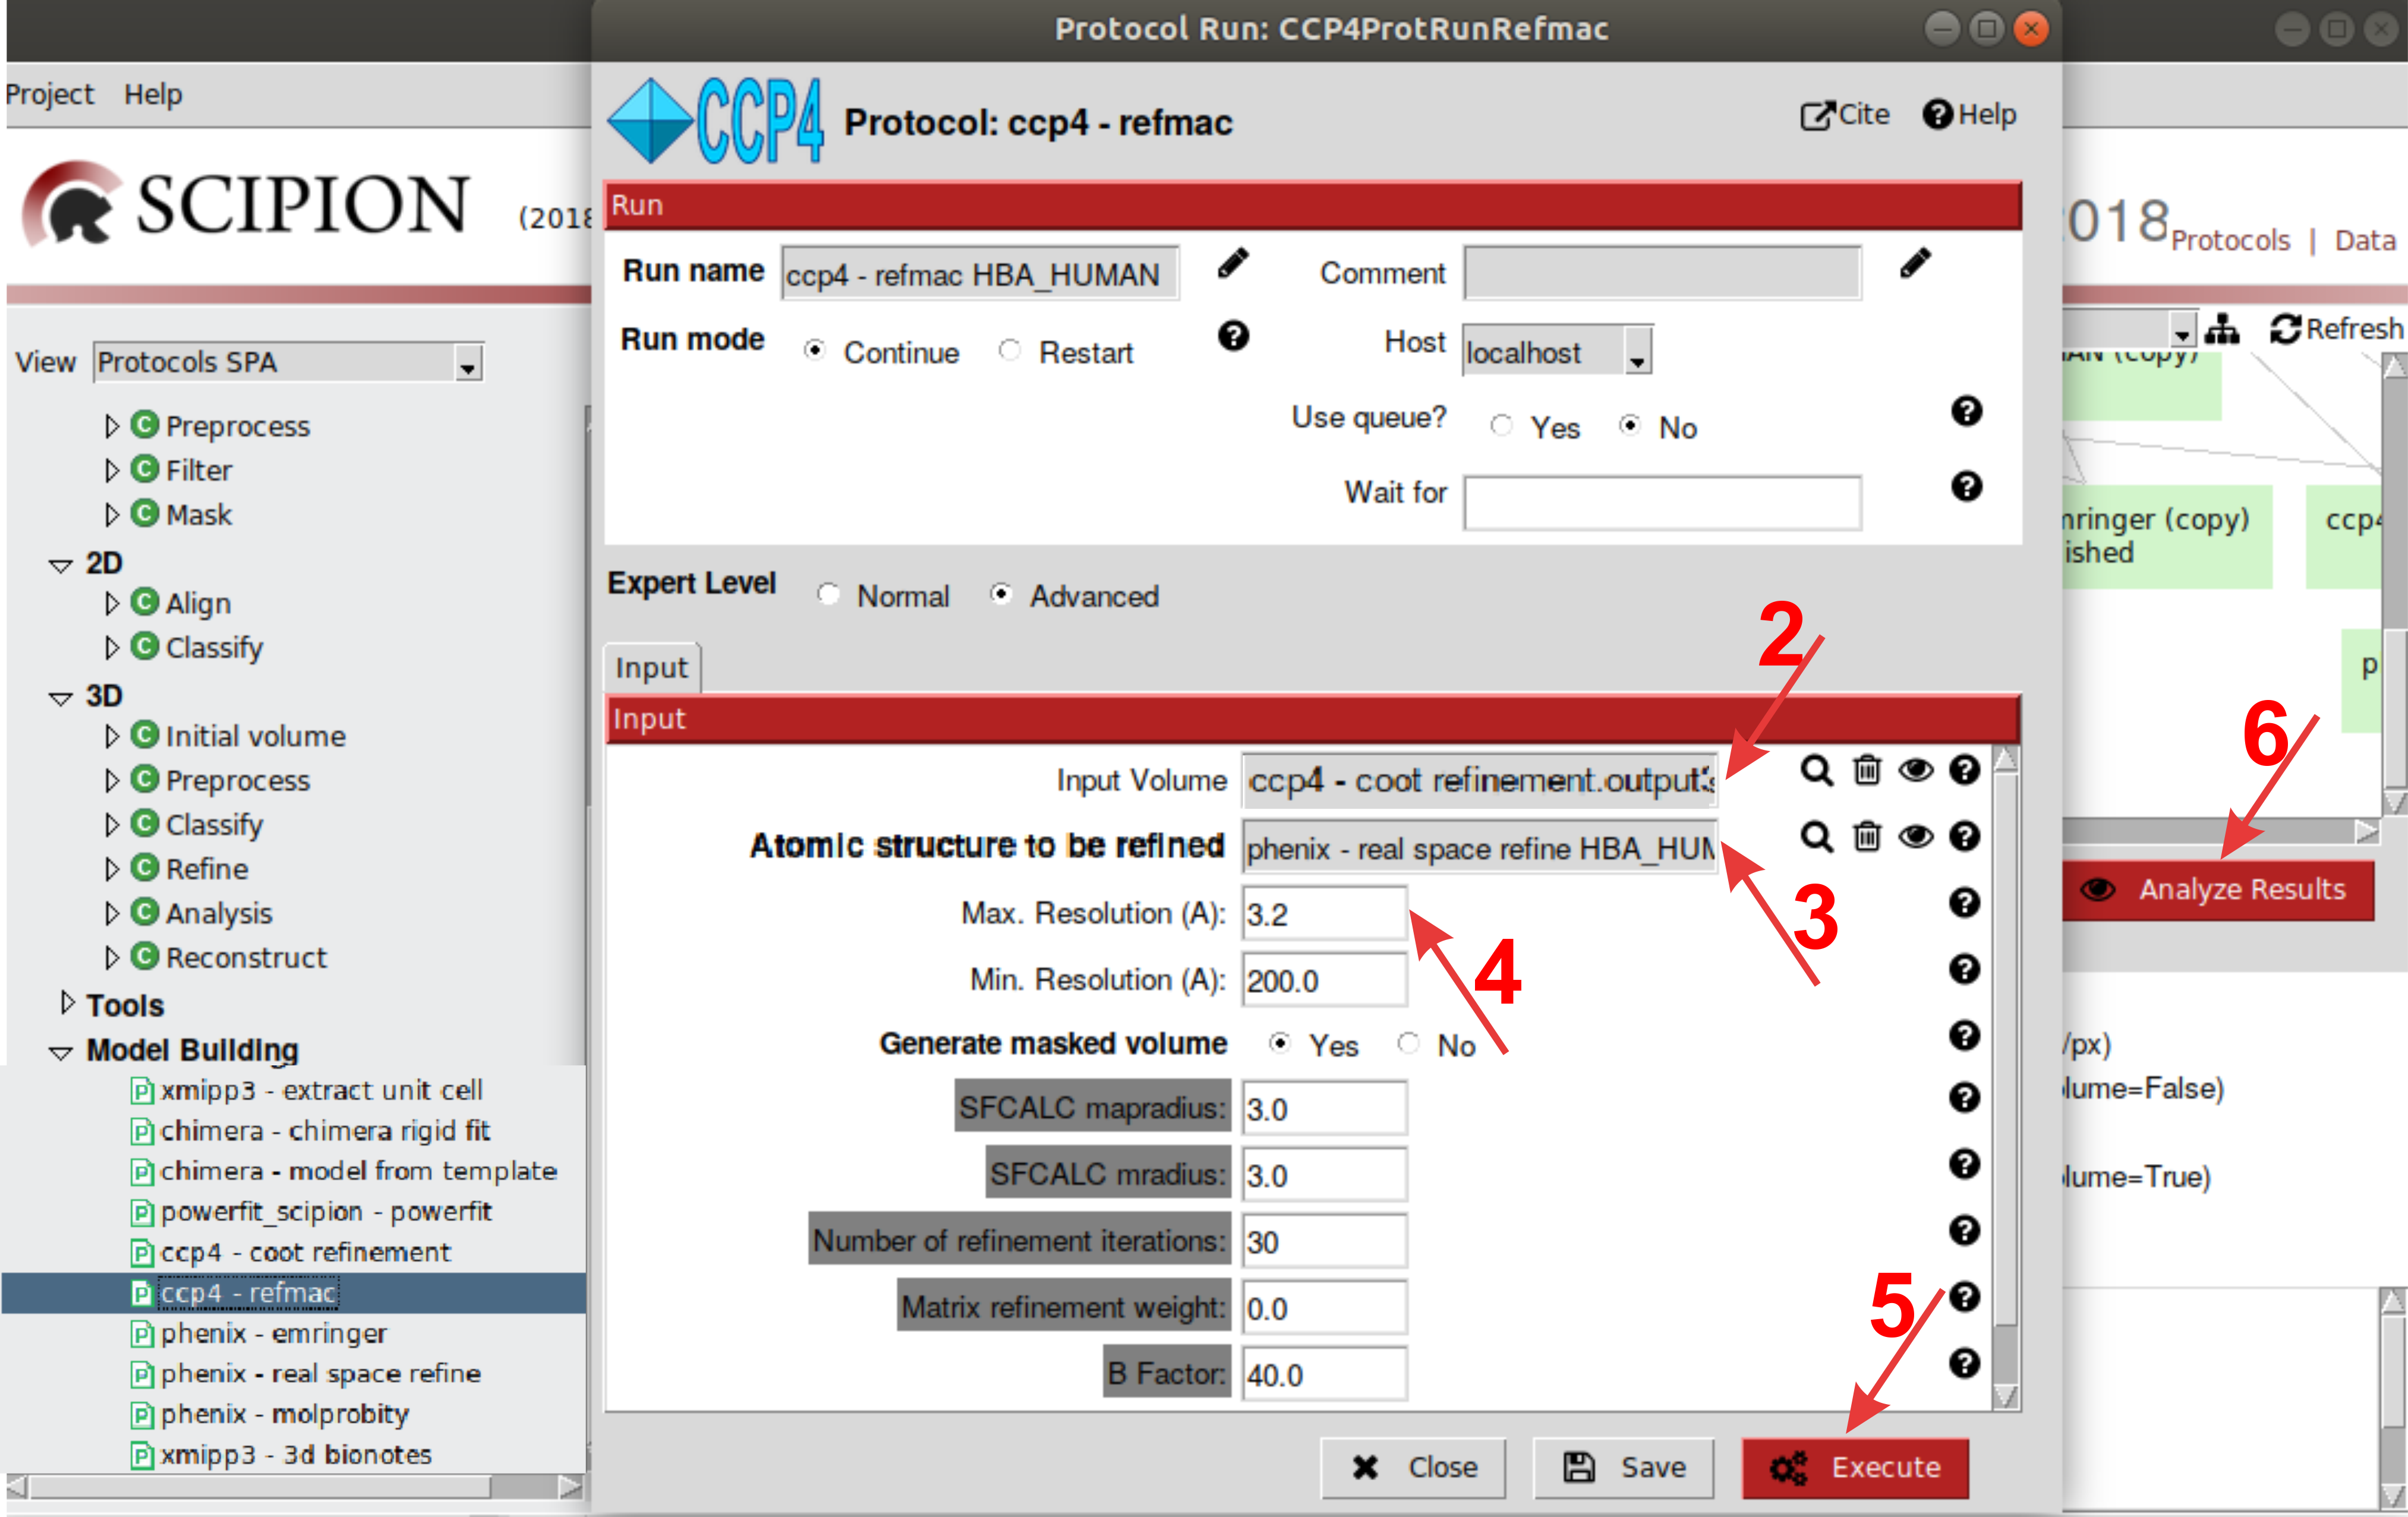
\includegraphics[width=0.85\textwidth]{Images/Fig31}
  \caption{Filling in \refmac protocol.}
  \label{fig:refmac_protocol}
  \end{figure}
  
  Clicking the first item in the display menu of results (\ffigure{fig:refmac_protocol} (1)), $Chimera$ graphics window will be opened showing the input volume, the initial $model$ (\ttt{HBA\_HUMAN} obtained with \phenix \ttt{real space refine}), and the final \refmac refined $model$ (\ffigure{fig:refmac_chimera}). By clicking the third item in the display menu of results (\ffigure{fig:refmac_protocol} (2)), a summary of \refmac results are shown. Check if values of \ttt{R factor} and \ttt{Rms BondLength} have improved with this refinement process. Why the improvement seems to be very small? (Answers in appendix \ref{app:solutions}; \textbf{Question 5})\\
  
  Would you have seen a higher improvement running \refmac immediately after \coot, thus ignoring $model$ improvements generated by \phenix \ttt{real space refine}? (Answers in appendix \ref{app:solutions}; \textbf{Question 6})\\
  
  Regarding the using of mask: Compare \refmac results (after \coot and \phenix \ttt{real space refine}) with those obtained selecting the option \ttt{No} in the protocol form parameter \ttt{Generate masked volume}. Use two different volumes, the one generated by \coot protocol, and the one generated by the \ttt{extract unit cell} protocol. Are there any differences? Why? (Answers in appendix \ref{app:solutions}; \textbf{Question 7})\\
  
  \begin{figure}[H]
  \centering 
  \captionsetup{width=.7\linewidth} 
  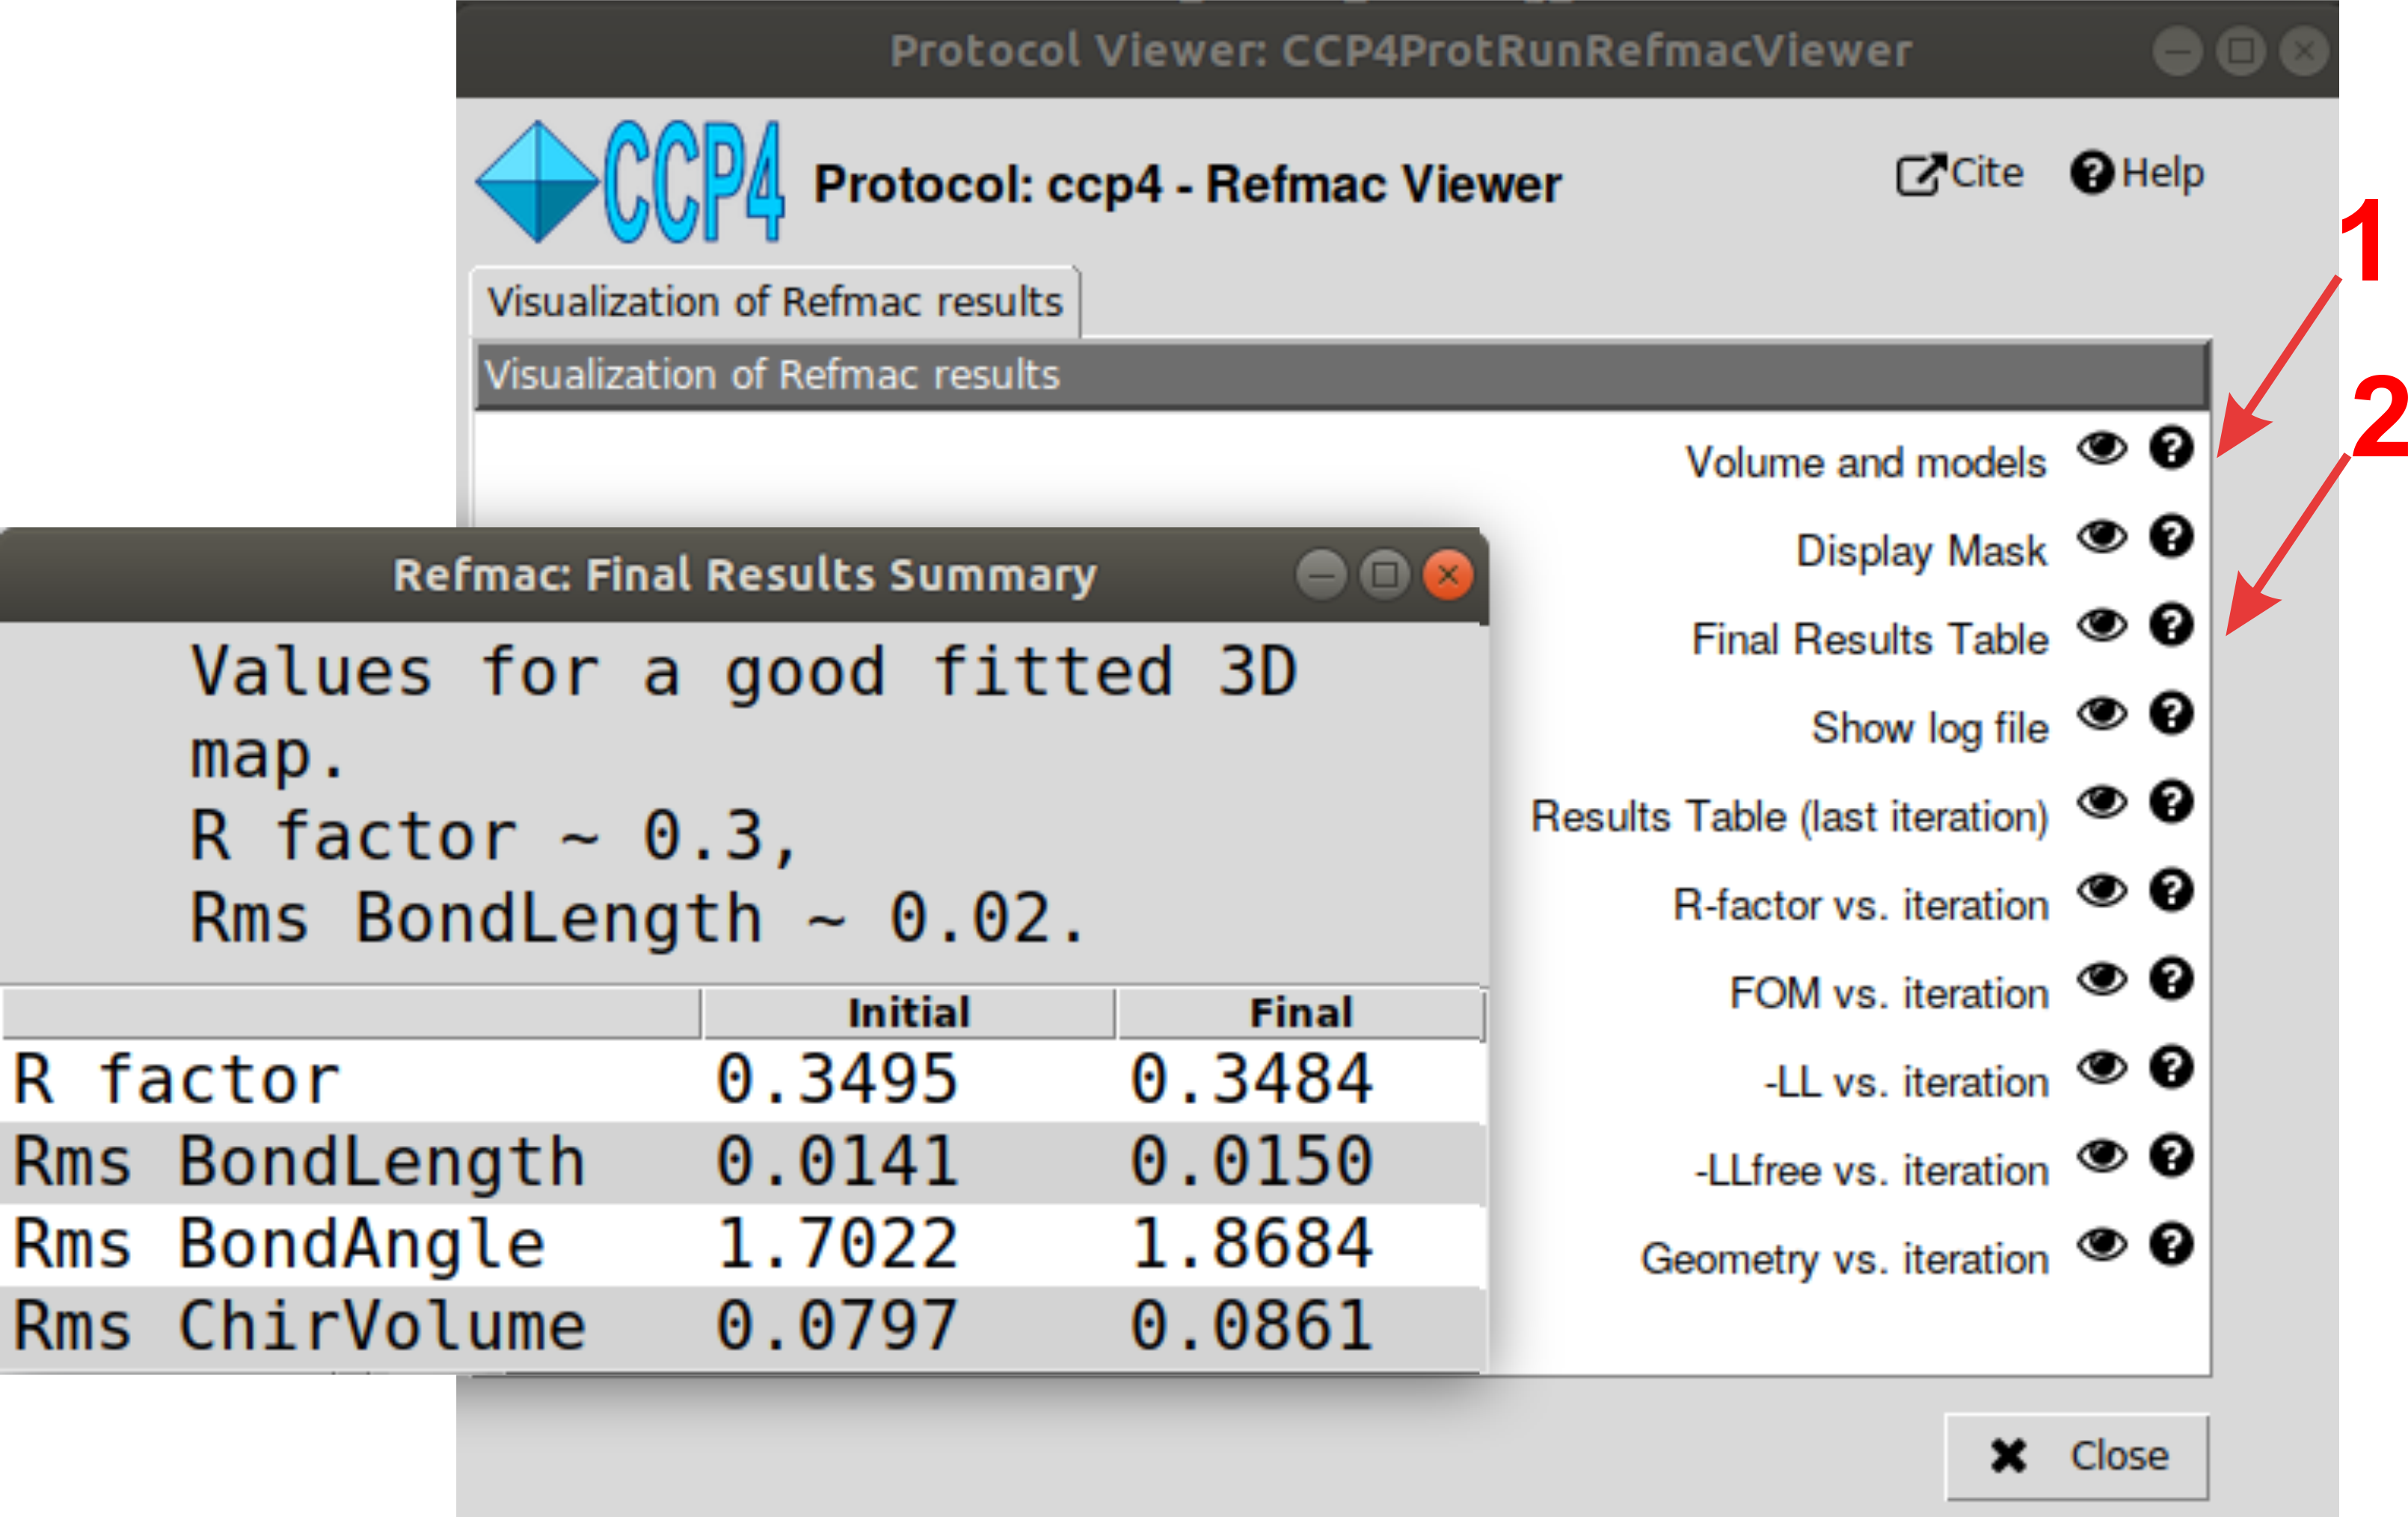
\includegraphics[width=0.85\textwidth]{Images/Fig32}
  \caption{Display menu of \refmac results.}
  \label{fig:refmac_display_results}
  \end{figure}
  
  \begin{figure}[H]
  \centering 
  \captionsetup{width=.7\linewidth} 
  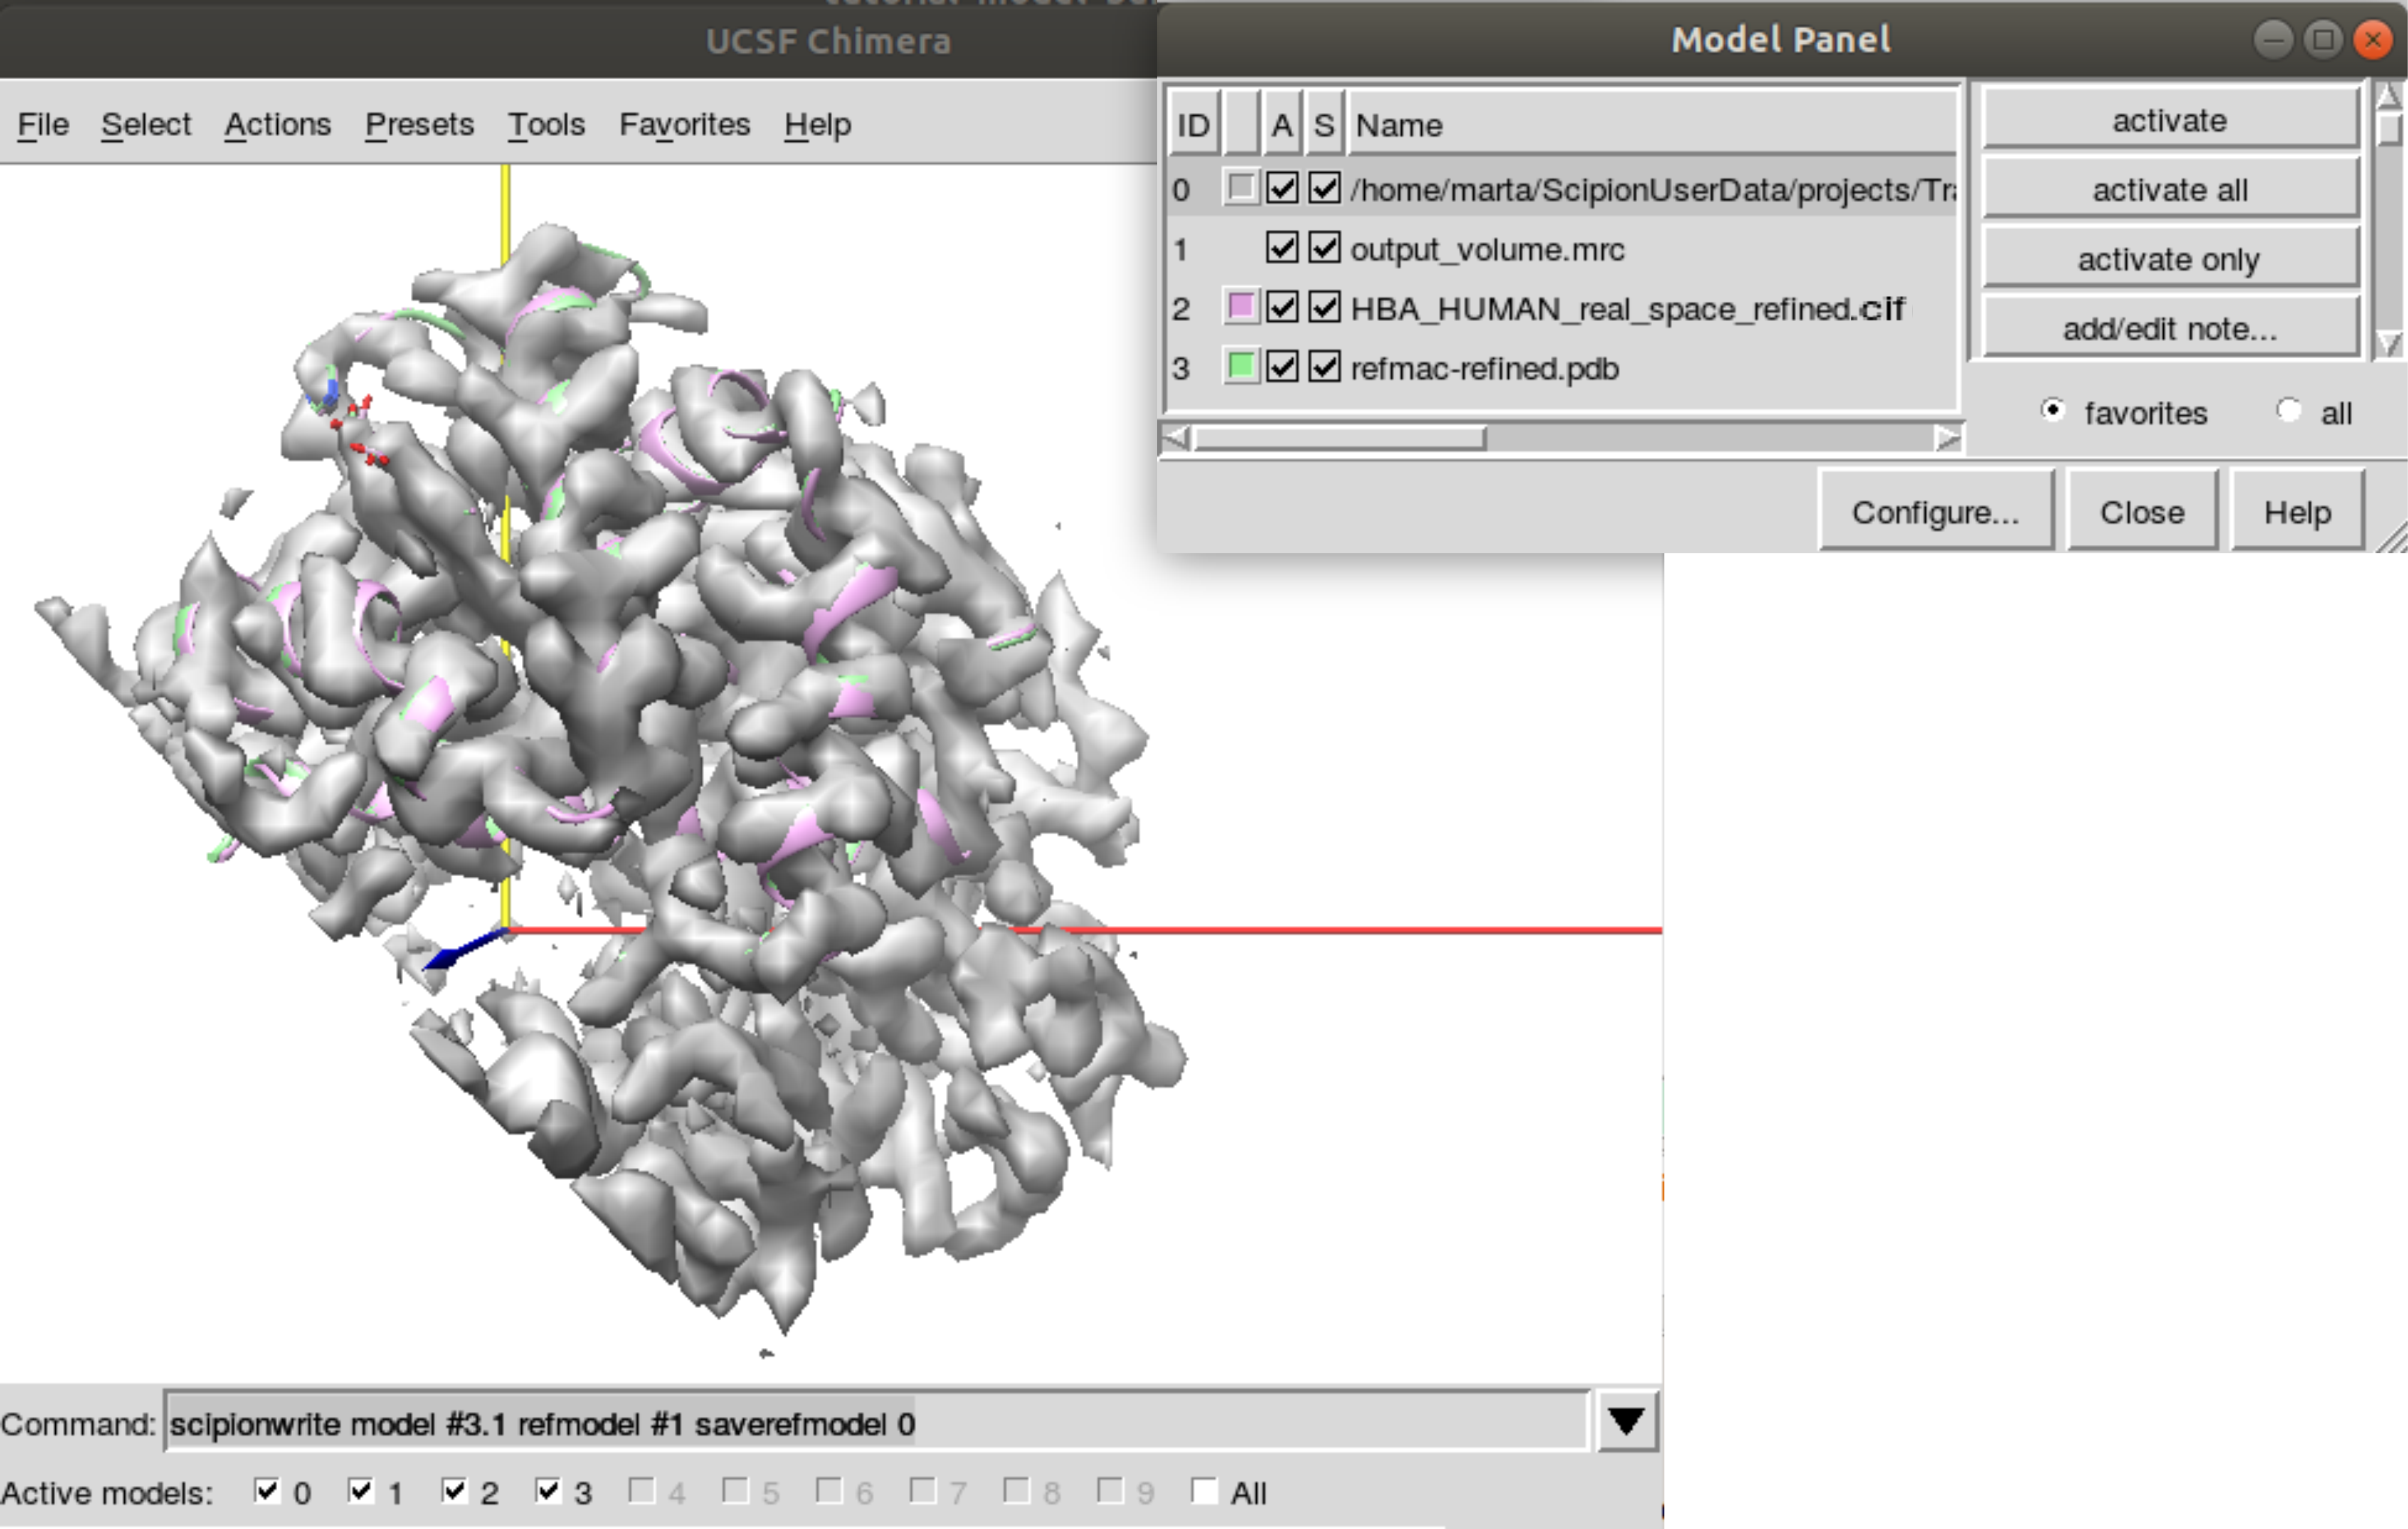
\includegraphics[width=0.85\textwidth]{Images/Fig33}
  \caption{$Chimera$ visualization of refined $model$ of \ttt{metHgb} $\alpha$ subunit by \refmac.}
  \label{fig:refmac_chimera}
  \end{figure}
  
  Have a look to the rest of items in the display window of results. 
  
